\documentclass[10pt,a4paper, margin=1in]{article}
\usepackage{fullpage}
\usepackage{amsfonts, amsmath, pifont}
\usepackage{amsthm}
\usepackage{graphicx}
\usepackage{float}

\usepackage{listings}

\usepackage{tkz-euclide}
\usepackage{tikz}
\usepackage{pgfplots}
\pgfplotsset{compat=1.13}

\usepackage{geometry}
 \geometry{
 a4paper,
 total={210mm,297mm},
 left=10mm,
 right=10mm,
 top=10mm,
 bottom=10mm,
 }
 % Write both of your names here. Fill exxxxxxx with your ceng mail address.
 \author{
  İşleyici, Osman Taylan\\
  \texttt{e2449496@ceng.metu.edu.tr}
  \and
  Deveci, Cengizhan\\
  \texttt{e2448322@ceng.metu.edu.tr}
}

\title{CENG 384 - Signals and Systems for Computer Engineers \\
Spring 2023 \\
Homework 3}
\begin{document}
\maketitle



\noindent\rule{19cm}{1.2pt}

\begin{enumerate}

\item %write the solution of q1
Let's say x(t) = $\sum_{k = -\infty}^{\infty}a_ke^{jkw_0t}$ \\

Integrate both side \\

$\int_{-\infty}^{t}x(s)ds = \int_{-\infty}^{t}\sum_{k = -\infty}^{\infty}a_ke^{jkw_0s}ds$ \\

$=\sum_{k = -\infty}^{\infty}\int_{-\infty}^{t}a_ke^{jkw_0s}ds = \sum_{k = -\infty}^{\infty}a_k\int_{-\infty}^{t}e^{jkw_0s}ds$ \\

$=\sum_{k = -\infty}^{\infty}a_k [\frac{e^{jkw_0s}}{jkw_0}|_{-\infty}^t]$ \\

$=\sum_{k = -\infty}^{\infty}a_k [\frac{e^{jkw_0t}}{jkw_0} - 0]$ \\

$=\sum_{k = -\infty}^{\infty}a_k \frac{e^{jkw_0t}}{jkw_0}$ \\

So the coefficients become $(\frac{1}{jkw_0})a_k$. $w_0 = \frac{2*\pi}{T}$. Thus, the coefficients is $(\frac{1}{jk\frac{2*\pi}{T}})a_k$

\item %write the solution of q2  
	\begin{enumerate}
    % Write your solutions in the following items.
    \item $\sum\limits_{\forall l}a_l*a_{k-l}$ because of the multiplication property of fourier series.
    \item Fourier series coefficient of even part of $x(t)$ is equal to real part of $a_k = \mathbb{R} \{a_k\}$.
	\item $x(t-t_0) = a_ke^{-jk(w\pi/T)t_0}$, $x(t+t_0) = a_ke^{jk(2\pi/T)t_0}$. $x(t-t_0) + x(t+t_0) = a_ke^{-jk(w\pi/T)t_0} + a_ke^{jk(2\pi/T)t_0}$.
    \end{enumerate}

\item %write the solution of q3

We know that $a_k = \frac{1}{T}\int_Tx(t)e^{-jkw_0t}dt$ \\

Let's take 1 period from -0.5 to 3.5. The period is 4 in this signal. We can write the $a_k$ as \\

$a_k = \frac{1}{T}\int_{-0.5}^{3.5}(2u(t) - 2u(t-1) - 2u(t-2) + 2u(t-3))e^{-jkw_0t}dt$ \\

$a_k = \frac{1}{T}(\int_{0}^{1}2e^{-jkw_0t}dt + \int_{1}^{2}0e^{-jkw_0t}dt + \int_{2}^{3}-2e^{-jkw_0t}dt + \int_{3}^{3.5}0e^{-jkw_0t}dt)$ \\

$\frac{1}{4} [(\frac{2e^{-jkw_0t}}{-jkw_0}|^1_0) + (\frac{-2e^{-jkw_0t}}{-jkw_0}|^3_2)]$ \\

$= \frac{1}{4} [(\frac{2e^{-jkw_0}}{-jkw_0}) - \frac{2}{-jkw_0} + (\frac{2e^{-jkw_0 3}}{jkw_0}) - (\frac{2e^{-jkw_0 2}}{jkw_0})]$ \\

$= \frac{1}{4} [\frac{-2e^{-jkw_0} + 2 + 2e^{-3jkw_0} - 2e^{-2jkw_0}}{jkw_0}]$ \\

$a_k = \frac{e^{-3jkw_0} - e^{-2jkw_0} -e^{jkw_0} + 1}{2jkw_0}$ \\

$x(t) = \sum_{k=-\infty}^{\infty}a_ke^{jkw_0t} = \sum_{k=-\infty}^{\infty}\frac{e^{-3jkw_0} - e^{-2jkw_0} -e^{-jkw_0} + 1}{2jkw_0}e^{-jkw_0t}$ \\

$= \sum_{k=-\infty}^{\infty}\frac{e^{-2jkw_0} - e^{-jkw_0} -e^{jkw_0} + 1}{2jkw_0}$

\item %write the solution of q4
    \begin{enumerate}   
    % Write your solutions in the following items.
    \item $sin(w_0t) = \frac{j}{2}(-e^{iw_0t} + e^{-iw_0t})$, $2*cos(w_0t) = e^{iw_0t} + e^{-iw_0t}$, $cos(2w_0t + \pi/4) = (e^{j\pi/4}*e^{2iw_0t} + e^{-2iw0t}/e^{j\pi/4})/2$ \\
    $a_{-2} = \frac{1}{2\sqrt{j}}$, since $\sqrt{j} = (1+j)/\sqrt{2}$, $a{-2} = \frac{1+j}{2\sqrt{2}}$\\
    $a_{-1} = j/2+1$\\
    $a_0 = 1$\\
    $a_1 = 1-j/2$\\
    $a_2 = \frac{1}{2\sqrt{j}} = \frac{\sqrt{2}}{2+2j}$\\

    \begin{tikzpicture}
        \begin{axis}[    xlabel={$k$},    ylabel={$|a_k|$},    axis lines=middle,    xmin=-2.5, xmax=2.5,    ymin=-0.1, ymax=1.5,    xtick={-2,-1,0,1,2},    ytick={0,0.5,1,1.118,1.5},    yticklabels={0,0.5,1,$\frac{\sqrt{5}}{2}$,1.5},    enlargelimits=true,    clip=false]
        \addplot [ycomb, black, thick, mark=*] table [x={k}, y={|a_k|}] {data4ai.dat};
        \end{axis}
        \end{tikzpicture}

        \begin{tikzpicture}
            \begin{axis}[    xlabel={$k$},    ylabel={$\angle a_k$},    axis lines=middle,
                    xmin=-2.5, xmax=2.5,    ymin=-1.5, ymax=1.5,    xtick={-2,-1,0,1,2},    
                    ytick={-0.7853, -0.5235, 0.5235, 0.7853},
                    yticklabels={$-\pi/4$, $-\pi/6$, $\pi/6$, $\pi/4$},]
            \addplot [ycomb, black, thick, mark=*] table [x={k}, y={angle}] {data4aii.dat};
            \end{axis}
            \end{tikzpicture}
    
    
    \item $\dot{y}(t) + y(t) = x(t)$, we should first find the particular solution of this system. We should write $x(t)$ as $e^{\lambda t}u(t)$ and $y(t)$ as $Kx(t)$ than solve the equation for K. $(\lambda K  + K)e^{\lambda t}u(t) = e^{\lambda t} u(t)$, $\lambda K + K = 1$, $K = \frac{1}{1+\lambda}$. The pole of transfer function is the eigenvalue of system. Which is -1 for this question.
	\item %write the solution of q4c
	$\frac{dy(t)}{dt} + y(t) = x(t)$ \\

    $y(t) = x(t) * h(t) = \int_{-\infty}^{\infty}x(\tau)h(t-\tau)d\tau$ \\

    $=\int_{-\infty}^{\infty}h(\tau)x(t-\tau)d\tau = \int_{-\infty}^{\infty}h(\tau)(\sum_{k}a_k e^{jkw_0 (t-\tau)}) d\tau$ \\

    $=\sum_{k}a_k e^{jkw_0 t}\int h(\tau)e^{-jkw_0 \tau} d\tau$ \\

    $=\sum_{k}a_k H(jkw_0)e^{jkw_0 t}$ \\

    $\sum_{k}a_k H(jkw_0)jkw_0 e^{jkw_0 t} + \sum_{k}a_k H(jkw_0) e^{jkw_0 t} = \sum_{k}a_k e^{jkw_0 t} $ \\

    $\sum_{k} a_k H(jkw_0)jkw_0 e^{jkw_0 t} + a_k H(jkw_0) e^{jkw_0 t} - a_k e^{jkw_0 t} = 0$\\

    $\sum_{k} a_k e^{jkw_0 t}(H(jkw_0) jkw_0 + H(jkw_0) - 1) = 0$ \\

    $H(jkw_0) = \frac{1}{jkw_0 + 1}$ \\

    $b_k = \frac{a_k}{jkw_0 + 1}$ \\
    \item %write the solution of q4d
    $y(t) = \sum_kb_ke^{jkw_0 t}$ \\
    
    $y(t) = \sum_k \frac{a_k e^{jkw_0 t}}{hkw_ 0 + 1}$
        
    \end{enumerate}

\item %write the solution of q5
    \begin{enumerate}
    % Write your solutions in the following items.
    \item %write the solution of q5a
    $x[n] = sin(\frac{\pi}{2}n)$ \\
    
    $x[n] = \frac{1}{2j}(e^{j\frac{\pi}{2}n} - e^{-j\frac{\pi}{2}n})$ Take $w_0 = \frac{\pi}{2}$ \\

    So $=> a_1 = \frac{1}{2j} $ and $a_{-1} = \frac{-1}{2j}$ \\

    $a_1 = \frac{1}{2j} = \frac{-j}{2}$ \\

    $a_{-1} = \frac{-1}{2j} = \frac{j}{2}$ \\

    \item %write the solution of q5b
    $y[n] = 1 + cos(\frac{\pi}{2}n)$ \\

    $= 1 + \frac{1}{2}(e^{j\frac{\pi}{2}n} + e^{-j\frac{\pi}{2}n})$ Take $w_0 = \frac{\pi}{2}$ \\

    $b_0 = 1$, $b_1 = b_{-1} = \frac{1}{2}$\\

	\item %write the solution of q5c
	$x[n] \longleftrightarrow^{F.S.} a_k$ \\

    $y[n] \longleftrightarrow^{F.S.} b_k$ \\

    $z[n] = x[n]y[n] \longleftrightarrow^{F.S.} c_k = \sum_{l=<N>}a_l b_{k-l}$ \\

    $c_k = \sum_{l = 0}^{3}a_l b_k-l$ since N = 4 \\

    $=a_0 b_k + a_1 b_{k-1} + a_2 b_{k-2} + a_3 b_{k-3} = a_1 b_{k-1} + a_3 b_{k-3}$ \\

    $c_0 = a_1 b_{-1} + a_3 b_{-3} = \frac{-j}{2}\frac{1}{2} + \frac{j}{2}\frac{1}{2} = 0$

    $c_1 = a_1 b_{0} + a_3 b_{-2} = \frac{-j}{2}1 + 0 = \frac{-j}{2}$

    $c_2 = a_1 b_{1} + a_3 b_{-1} = \frac{-j}{2}\frac{1}{2} + \frac{j}{2}\frac{1}{2} = 0$

    $c_3 = a_1 b_{2} + a_3 b_{0} = \frac{-j}{2}0 + \frac{j}{2}1 = \frac{j}{2}$
	\item %write the solution of q5d
	$x[n]y[n] = \sin(\frac{\pi}{2}n)(1 + cos(\frac{\pi}{2}n))$ \\

    $= sin(\frac{\pi}{2}n) + sin(\frac{\pi}{2}n) cos(\frac{\pi}{2}n) = sin(\frac{\pi}{2}n) + \frac{sin\pi n}{2}$ and $ sin\pi n$ is zero. Therefore \\

    $= sin(\frac{\pi}{2}n)$\\

    like part a\\

    $z[n] = \frac{1}{2j}(e^{j\frac{\pi}{2}n} - e^{-j\frac{\pi}{2}n})$\\

    $c_1 = \frac{-j}{2}$ and $c_{-1} = c_{3} = \frac{j}{2}$. So as expected the result is the same with part c.
    \end{enumerate}    
    
\item %write the solution of q6
    \begin{enumerate}
    % Write your solutions in the following items.
    \item We can see that the period of this signal is 4. We can then we can use the analysis formula to find fourier coefficients.\\ 
    $a_k = \frac{1}{4}\sum\limits_{n=0}^{3}x[n]e^{-jk(\pi/2)n}$\\
    $a_k = \frac{1}{4}(0+e^{-jk\pi/2} + 2e^{-jk\pi} + e^{-3jk\pi/2})$ \\
    $e^{jk\pi/2} = j$ so\\
    $a_0 = 1$\\
    $a_1 = -1/2$\\
    $a_2 = 0$\\
    $a_3 = -1/2$
    From periodicity of signal, we can say that $a_k$ does also have period 4.\\
    \begin{filecontents}{data6a.dat}
        k    a_k
        -4   1
        -3   0.5
        -2   0
        -1   0.5
        0    1
        1    0.5
        2    0
        3    0.5
        4    1
    \end{filecontents}\\
    \begin{tikzpicture}
        \begin{axis}[
          xlabel={$n$},
          ylabel={$x[n]$},
          axis lines=middle,
          ymax=1.5,
          xmin=-4, xmax=4,
          ymin=-0.3, ymax=1.5,
          ytick={-1, -0.5, 0, 0.5, 1},
          ]
          \addplot [ycomb, black, thick, mark=*] table [x={k}, y={a_k}] {data6a.dat};
        \end{axis}
        \end{tikzpicture}
    \item If we examine the graph, we can see that this signal is $y[n] = x[n]x[n-1]$.\\
    We can use difference and multiplication properties to find the spectral coefficients of Fourier series. \\
    $x[n+1] \leftrightarrow c_k = a_ke^{jk\pi/2} = \frac{1}{4}(e^{jk\pi}+2e^{jk\pi/2}+1)$\\
    $x[n]x[n+1] \leftrightarrow b_k=\sum\limits_{l=0}^4 a_lc_{k-l}$\\
    Or we can just use the analysis formula instead of calculating this sum.\\
    $b_k = \frac{1}{4}\sum\limits_{n=0}^4y[n]e^{-jk(\pi/2)(n-2)}$\\
    $b_k = \frac{1}{4}(e^{jk\pi/2}+2)$\\
    $e^{j\pi/2} = j$\\
    $b_0 = 3/4$\\
    $b_1 = \frac{j+2}{4}$\\
    $b_2 = 1/4$\\
    $b_3= \frac{4-j}{2}$.

    \end{enumerate}
    
\item %write the solution of q7
    \begin{enumerate}
    % Write your solutions in the following items.
    \item %write the solution of q7a
    In CT LTI system \\

    $e^{st} \rightarrow H(s)e^{st}$ \\

    $= e^{st} \int_{-\infty}^{\infty}h(\tau)e^{-s\tau}d\tau$. \\
    
    $y(jw) = x(jw) * H(jw)$. \\
    
    If y(t) = x(t). We can say that y(jw) = x(jw). Then we can say that the coefficients should be identical.

    That implies that system does not change in any value. It can be possible if the transfer function H = 1 so that $|w| \leq 80$.

    \item %write the solution of q7b
    In contrary to part a. If the $y(t) \neq x(t)$ then there should be some values w where the transfer function not equal to 1. As a result we can say that for w that there should be some values of w that $|w| > 80$.
    \end{enumerate}    
	
\item %write the solution of q8	
    \begin{enumerate}
        \item 
        ~\\
        \begin{figure}[H]
            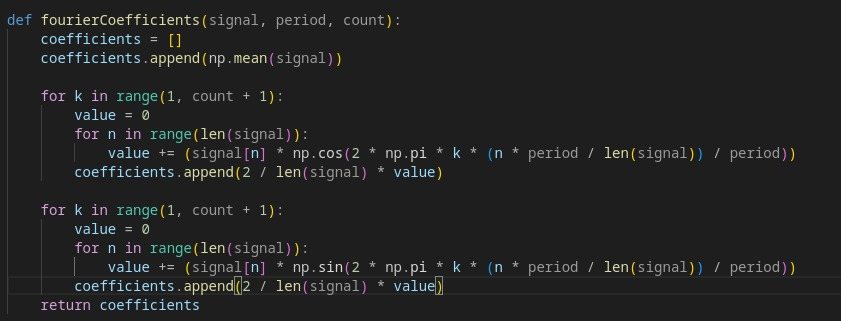
\includegraphics[scale=0.75]{fourierCoefFunc.jpeg}
            \caption{Fourier Coefficients Calculate function}
        \end{figure}
        \item 
        ~\\
        \begin{figure}[H]
            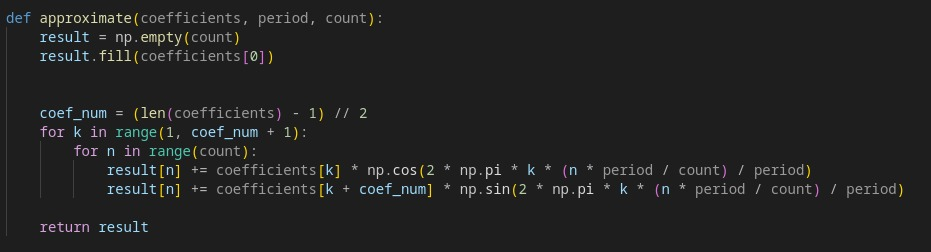
\includegraphics[scale=0.75]{approximateFunc.jpeg}
            \caption{Approximation function}
        \end{figure}
        \item 
        ~\\
        \begin{figure}[H]
            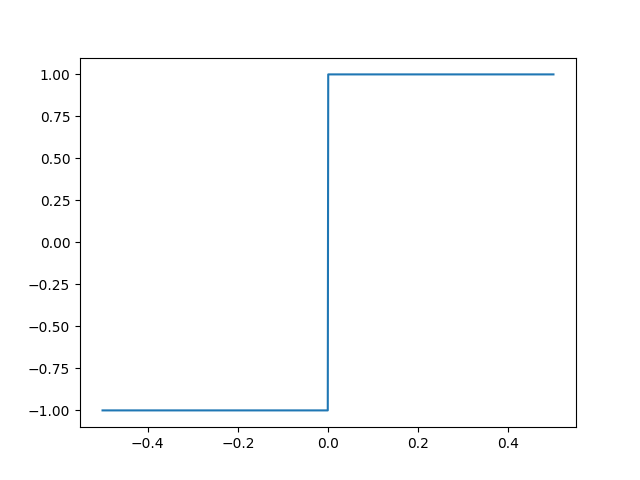
\includegraphics[scale=0.75]{originalSignal.png}
            \caption{Original signal}
        \end{figure}

        \begin{figure}[H]
            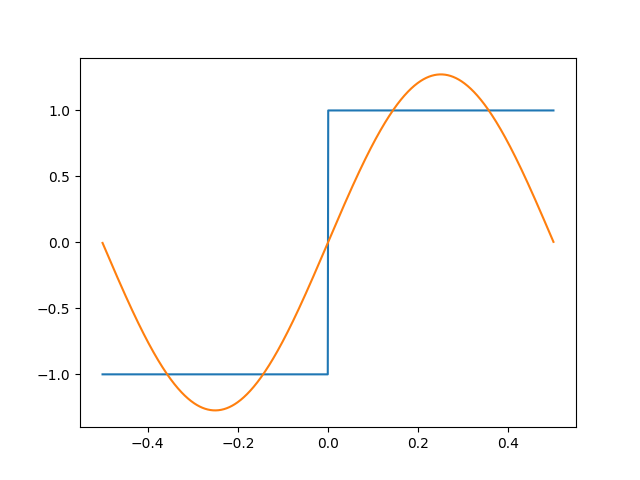
\includegraphics[scale=0.75]{approximated_n=1.png}
            \caption{Approximated signal n = 1}
        \end{figure}
        \begin{figure}[H]
            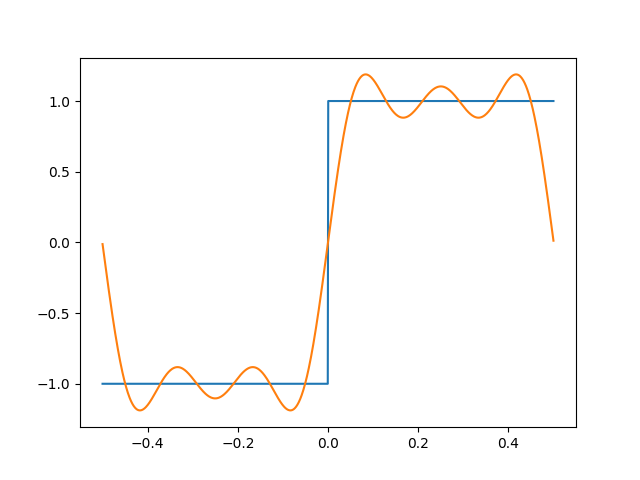
\includegraphics[scale=0.75]{approximated_n=5.png}
            \caption{Approximated signal n = 5}
        \end{figure}
        \begin{figure}[H]
            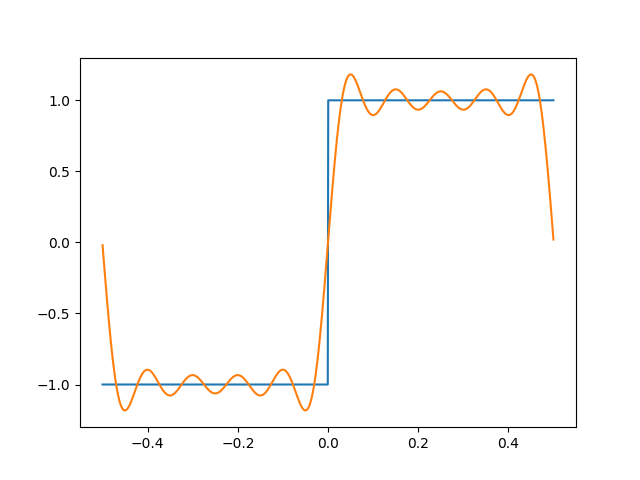
\includegraphics[scale=0.75]{approximated_n=10.png}
            \caption{Approximated signal n = 10}
        \end{figure}
        \begin{figure}[H]
            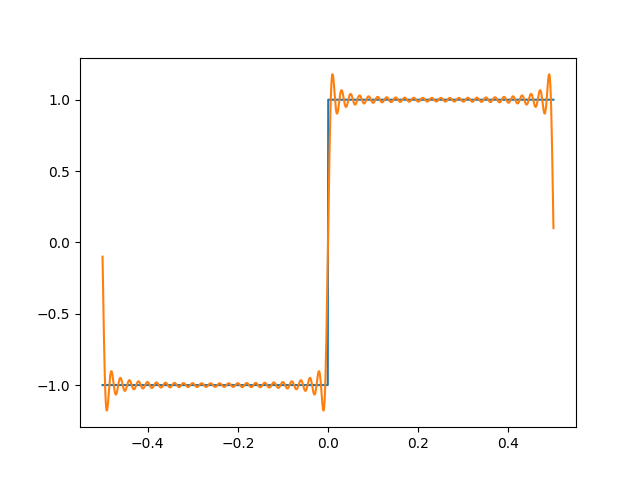
\includegraphics[scale=0.75]{approximated_n=50.png}
            \caption{Approximated signal n = 50}
        \end{figure}
        \begin{figure}[H]
            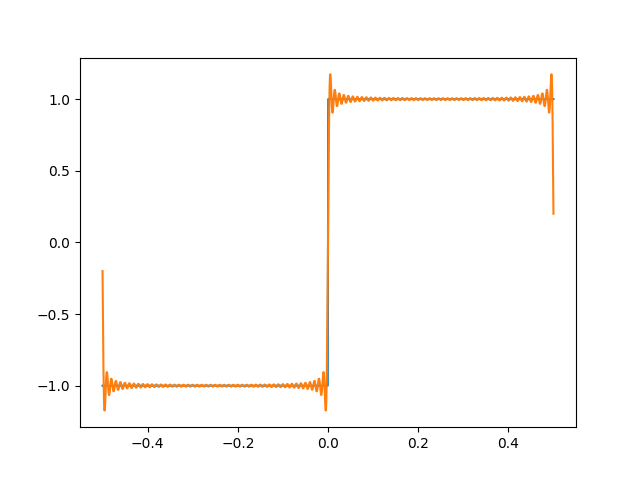
\includegraphics[scale=0.75]{approximated_n=100.png}
            \caption{Approximated signal n = 100}
        \end{figure}
        \item 
        ~\\
        \begin{figure}[H]
            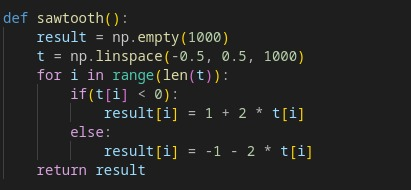
\includegraphics[scale=0.75]{sawToothFunc.jpeg}
            \caption{Sawtooth function}
        \end{figure}
        \begin{figure}[H]
            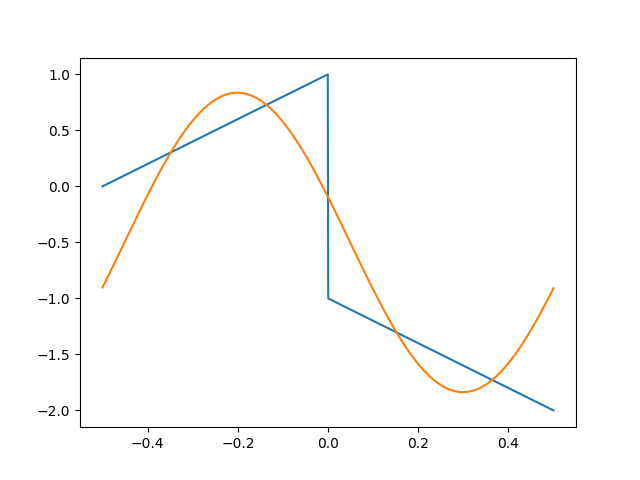
\includegraphics[scale=0.75]{approximatedSaw_n=1.png}
            \caption{Approximated Saw signal n = 1}
        \end{figure}
        \begin{figure}[H]
            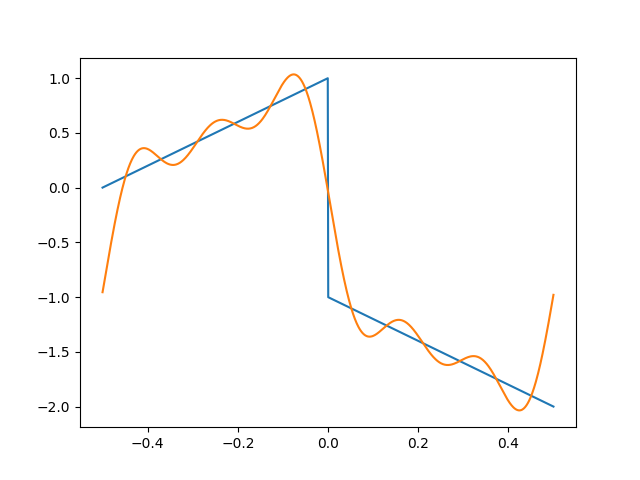
\includegraphics[scale=0.75]{approximatedSaw_n=5.png}
            \caption{Approximated Saw signal n = 5}
        \end{figure}
        \begin{figure}[H]
            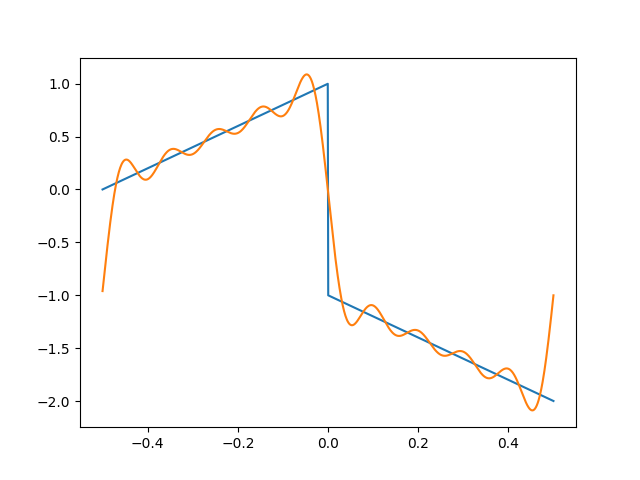
\includegraphics[scale=0.75]{approximatedSaw_n=10.png}
            \caption{Approximated Saw signal n = 10}
        \end{figure}
        \begin{figure}[H]
            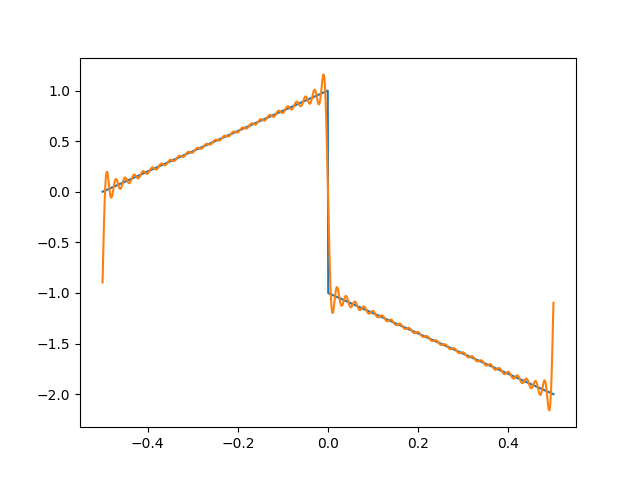
\includegraphics[scale=0.75]{approximatedSaw_n=50.png}
            \caption{Approximated Saw signal n = 50}
        \end{figure}
        \begin{figure}[H]
            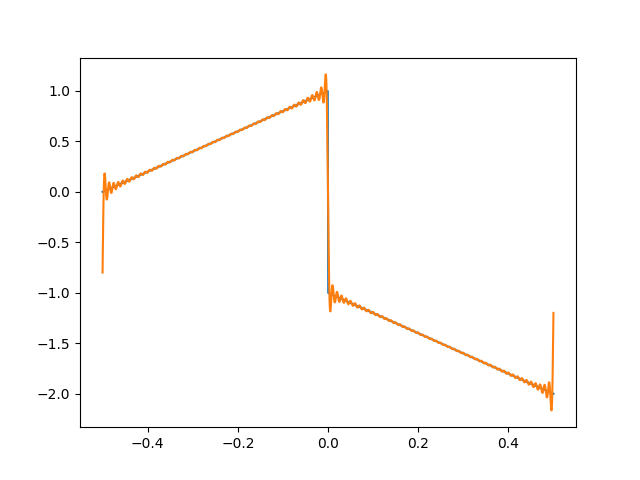
\includegraphics[scale=0.75]{approximatedSaw_n=100.png}
            \caption{Approximated Saw signal n = 100}
        \end{figure}
        When we increase the n, the result will become more as expected signal.
    \end{enumerate}

    \lstset{language=Python}
    \lstset{frame=single}
    \lstset{caption={Solution code}}
    \lstset{label={lst:code_direct}}
    \lstset{basicstyle=\footnotesize}
    \begin{lstlisting}
    import matplotlib.pyplot as plt
    import numpy as np
    import scipy.signal as sp

    def fourierCoefficients(signal, period, count):
        coefficients = []
        coefficients.append(np.mean(signal))

        for k in range(1, count + 1):
            value = 0
            for n in range(len(signal)):
                value += (signal[n] * np.cos(2 * np.pi * k * (n * period / len(signal)) / period))
            coefficients.append(2 / len(signal) * value)

        for k in range(1, count + 1):
            value = 0
            for n in range(len(signal)):
                value += (signal[n] * np.sin(2 * np.pi * k * (n * period / len(signal)) / period))
            coefficients.append(2 / len(signal) * value)
        return coefficients

    def approximate(coefficients, period, count):
        result = np.empty(count)
        result.fill(coefficients[0])


        coef_num = (len(coefficients) - 1) // 2
        for k in range(1, coef_num + 1):
            for n in range(count):
                result[n] += coefficients[k] * np.cos(2 * np.pi * k * (n * period / count) / period)
                result[n] += coefficients[k + coef_num] * np.sin(2 * np.pi * k * (n * period / count) / period)
        
        return result

    def sawtooth():
        result = np.empty(1000)
        t = np.linspace(-0.5, 0.5, 1000)
        for i in range(len(t)):
            if(t[i] < 0):
                result[i] = 1 + 2 * t[i]
            else:
                result[i] = -1 - 2 * t[i]
        return result

    def main():
        signal = []
        for i in range(500):
            signal.append(-1)
        for i in range(500):
            signal.append(1)

        plt.plot(np.linspace(-0.5, 0.5, 1000), signal, label='Original')
        plt.show()

        coef = fourierCoefficients(signal, 1, 1)
        approximation = approximate(coef, 1, 1000)
        plt.plot(np.linspace(-0.5, 0.5, 1000), signal, label='Original')
        plt.plot(np.linspace(-0.5, 0.5, 1000), approximation, label='Approximation')
        plt.show()

        coef = fourierCoefficients(signal, 1, 5)
        approximation = approximate(coef, 1, 1000)
        plt.plot(np.linspace(-0.5, 0.5, 1000), signal, label='Original')
        plt.plot(np.linspace(-0.5, 0.5, 1000), approximation, label='Approximation')
        plt.show()

        coef = fourierCoefficients(signal, 1, 10)
        approximation = approximate(coef, 1, 1000)
        plt.plot(np.linspace(-0.5, 0.5, 1000), signal, label='Original')
        plt.plot(np.linspace(-0.5, 0.5, 1000), approximation, label='Approximation')
        plt.show()


        coef = fourierCoefficients(signal, 1, 50)
        approximation = approximate(coef, 1, 1000)
        plt.plot(np.linspace(-0.5, 0.5, 1000), signal, label='Original')
        plt.plot(np.linspace(-0.5, 0.5, 1000), approximation, label='Approximation')
        plt.show()

        coef = fourierCoefficients(signal, 1, 100)
        approximation = approximate(coef, 1, 1000)
        plt.plot(np.linspace(-0.5, 0.5, 1000), signal, label='Original')
        plt.plot(np.linspace(-0.5, 0.5, 1000), approximation, label='Approximation')
        plt.show()

        signalSaw = sawtooth()

        coef = fourierCoefficients(signalSaw, 1, 1)
        approximation = approximate(coef, 1, 1000)
        plt.plot(np.linspace(-0.5, 0.5, 1000), signalSaw, label='Original')
        plt.plot(np.linspace(-0.5, 0.5, 1000), approximation, label='Approximation')
        plt.show()

        coef = fourierCoefficients(signalSaw, 1, 5)
        approximation = approximate(coef, 1, 1000)
        plt.plot(np.linspace(-0.5, 0.5, 1000), signalSaw, label='Original')
        plt.plot(np.linspace(-0.5, 0.5, 1000), approximation, label='Approximation')
        plt.show()

        coef = fourierCoefficients(signalSaw, 1, 10)
        approximation = approximate(coef, 1, 1000)
        plt.plot(np.linspace(-0.5, 0.5, 1000), signalSaw, label='Original')
        plt.plot(np.linspace(-0.5, 0.5, 1000), approximation, label='Approximation')
        plt.show()


        coef = fourierCoefficients(signalSaw, 1, 50)
        approximation = approximate(coef, 1, 1000)
        plt.plot(np.linspace(-0.5, 0.5, 1000), signalSaw, label='Original')
        plt.plot(np.linspace(-0.5, 0.5, 1000), approximation, label='Approximation')
        plt.show()

        coef = fourierCoefficients(signalSaw, 1, 100)
        approximation = approximate(coef, 1, 1000)
        plt.plot(np.linspace(-0.5, 0.5, 1000), signalSaw, label='Original')
        plt.plot(np.linspace(-0.5, 0.5, 1000), approximation, label='Approximation')
        plt.show()

    if __name__ == "__main__":
        main()
                        
    \end{lstlisting}
\end{enumerate}




\end{document}

